\chapter{System Analysis}

\section{Use Cases}

\section{State Machine}
Since a real-time processing could not be realised this section contains a theoretically fitting state-machine and an activity diagram explaining the different stages of the application. In figure \ref{statemachine} the theoretical state machine can be seen.

\begin{figure}[H]
	\centering
	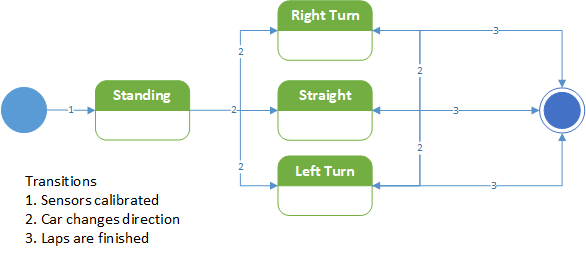
\includegraphics[scale=0.8]{Pictures/statemachine.png}
	\caption{Theoretical state machine}
	\label{statemachine}
\end{figure}

The flow the application is taking, is demonstrated in figure \ref{activitydiagram}. It can be seen that the user has two different options. First, a new session can be started, which is followed by positioning the car and calibrate the sensors. The other option is to review previous sessions. Therefore the user must select one of the stored data sets. When choosing a new session, the start of the race is triggered, when the car leaves the start. The race finish is triggered by pressing a button. The next step is the same for both decisions of the user. The data set, new or old, is taken and analysed. This is done to provide backward compatibility, when updates are rolled out. After the data has been processed, the report is created with tips for performance improvement.

\begin{figure}[H]
	\centering
	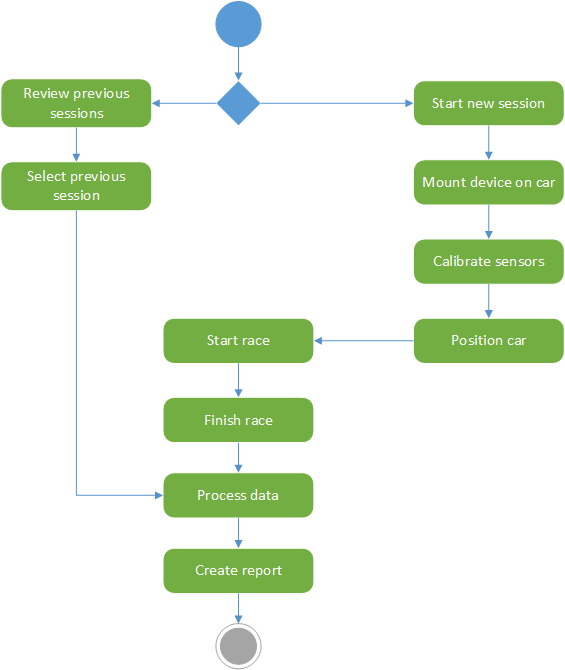
\includegraphics[scale=0.8]{Pictures/activitydiagram.png}
	\caption{Activity diagram of LapOps}
	\label{activitydiagram}
\end{figure}